% Insert in the relevant Methods subsection; compile from overleaf/SWBAM/.
\begin{figure*}[!t]
    \centering
    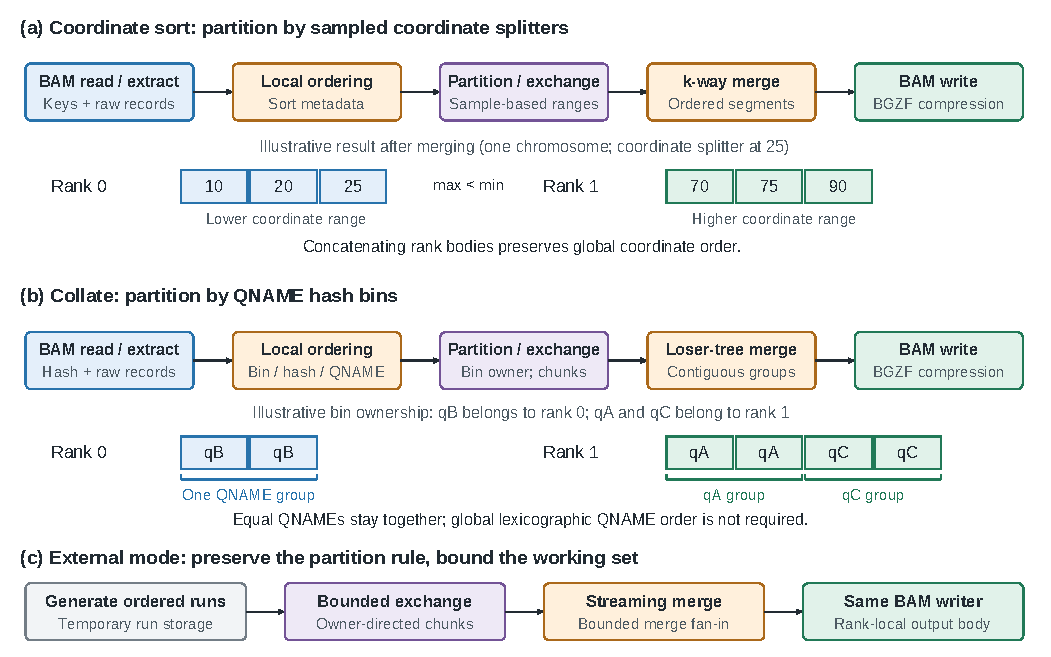
\includegraphics[width=\textwidth]{../figs/swbam_distributed_reordering.pdf}
    \caption{Distributed reordering built on the common BAM read and
    write pipelines. (a) Sort orders local metadata, chooses coordinate
    splitters from samples, redistributes records by coordinate range, and
    merges ordered source segments. (b) Collate routes QNAME hash bins to owner
    ranks and merges records into contiguous QNAME groups. Its ordering is
    based on bin/hash and QNAME, not global QNAME lexicographic order. Toy
    outputs illustrate the different ordering guarantees, not actual datasets
    or sampled splitters. (c) External-memory variants preserve their
    partitioning rules while using ordered runs, bounded exchanges and
    streaming merges. Algorithmic run files are distinct from output-body
    spool files.}
    \label{fig:swbam_distributed_reordering}
\end{figure*}
